
%(BEGIN_QUESTION)
% Copyright 2006, Tony R. Kuphaldt, released under the Creative Commons Attribution License (v 1.0)
% This means you may do almost anything with this work of mine, so long as you give me proper credit

Thermocouple wire can be quite expensive in some cases.  Suppose a technician is tempted to save money, and decides to use a copper wire pair to span the distance between the thermocouple ``head'' and the control room where the indicating instrument is located, instead of thermocouple wire or thermocouple extension wire:

$$\includegraphics[width=15.5cm]{i00374x01.eps}$$

Drawn in more of a schematic diagram form, the circuit looks like this:

$$\includegraphics[width=15.5cm]{i00374x02.eps}$$

Explain why this attempt to save money is a bad idea.

\underbar{file i00374}
%(END_QUESTION)





%(BEGIN_ANSWER)

The connections made inside the thermocouple head form a reference junction, the temperature of which will subtract from the furnace's temperature to yield the total voltage registered by the instrument room indicator.

%(END_ANSWER)





%(BEGIN_NOTES)


%INDEX% Measurement, temperature: thermocouple

%(END_NOTES)


